\documentclass{article}

\usepackage[spanish]{babel}
\usepackage[utf8]{inputenc}
\usepackage[right=1.5cm,left=1.5cm,top=1.5cm,bottom=1.5cm]{geometry}

\title{Taller 3A\\ Estadística genómica}
\author{Juan David Henao Sánchez}

\usepackage{Sweave}
\begin{document}
\Sconcordance{concordance:JuanHenao_Taller3A.tex:JuanHenao_Taller3A.Rnw:%
1 9 1 1 0 9 1 1 2 1 0 1 1 3 0 2 2 1 0 1 1 5 0 1 1 19 0 2 2 5 0 2 2 1 0 %
2 1 11 0 2 1 3 0 2 2 1 0 1 1 7 0 2 2 20 0 2 2 1 0 2 1 19 0 2 2 5 0 2 2 %
1 0 1 1 5 0 1 1 11 0 1 2 2 1}


\maketitle

\section*{Sobre unos datos del GEO (una sola medición en el tiempo) que comparen dos condiciones, identifique los genes diferencialmente expresados usando acde:
}

\begin{Schunk}
\begin{Sinput}
> library(acde)
> library("DESeq")
> #########################
> data <- read.table("GSE55477_GeneExpression_RPKMs.txt", h=T)
> dim(data)
\end{Sinput}
\begin{Soutput}
[1] 13321     9
\end{Soutput}
\begin{Sinput}
> head(data)
\end{Sinput}
\begin{Soutput}
      GeneID Chromosome Gene_length Spores_Rep_1 Spores_Rep_2 Spores_Rep_3
1 FGSG_11641     Fgchr1         666            0            0            0
2 FGSG_11605     Fgchr1        1134         0.11            0            0
3 FGSG_11642     Fgchr1         669         1.68         2.26         3.14
4 FGSG_11643     Fgchr1         396            0            0            0
5 FGSG_11600     Fgchr1        1305         0.96         0.62         0.54
6 FGSG_11601     Fgchr1         423         0.59         0.55         0.28
  Mycelium_Rep_1 Mycelium_Rep_2 Mycelium_Rep_3
1              0              0           0.00
2           0.25              0           0.16
3           0.64           1.56           3.47
4              0              0           0.00
5           0.22           0.11           0.41
6              0              0           0.00
\end{Soutput}
\end{Schunk}
\begin{Schunk}
\begin{Sinput}
> boxplot(data[, 4:9], main="Boxplot Fusarium graminearum", col="lightgreen", cex.names=0.2, las=2)
\end{Sinput}
\end{Schunk}
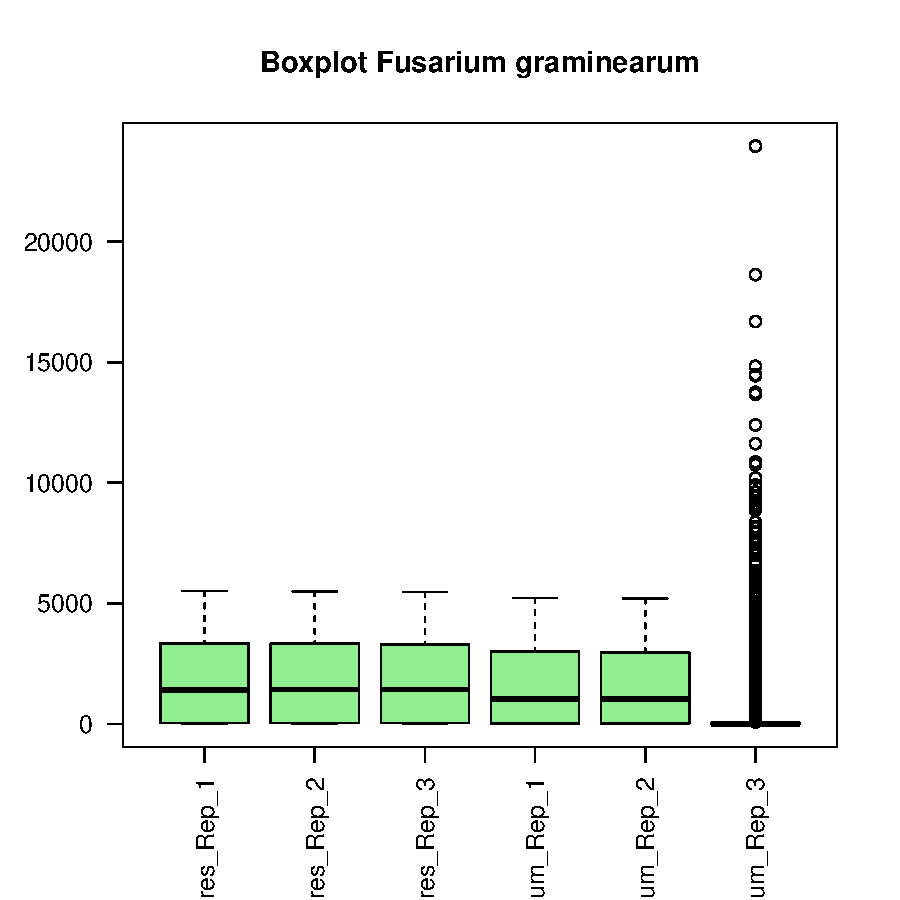
\includegraphics{JuanHenao_Taller3A-002}
\begin{Schunk}
\begin{Sinput}
> rownames(data) <- data$GeneID
\end{Sinput}
\end{Schunk}

\end{document}
